\section[The inverse function theorem]{The inverse function theorem}
\paragraph{Motivation}
In analysis of functions in one variable we had that
\begin{thm}
Given
\begin{enumerate}
  \item $f: I \rightarrow \RR.\ I \subset \RR$ ($I$ being an open interval)
  \item $f$ is continuously differentiable on its domain $I$
  \item $f'(x) \neq 0\  \forall x \in I$ (i.e. $f$ is strictly increasing or decreasing)
\end{enumerate}
Then $f$ is invertible (injective), its inverse $f^{-1}$ is also continuously differentiable and
$$(f^{-1})'(f(x)) = \frac{1}{f'(x)}$$
\end{thm}

\begin{rem}
  Can be derived as $$f^{-1}(f(x)) = x\ \underrightarrow{^\text{differentiate}}\ (f^{-1})'(f(x)).f'(x) = 1 \iff (f^{-1})'(f(x)) = \frac{1}{f'(x)}$$
  \end{rem}

\begin{figure}[hb]
  \center
\caption{Geometric idea of inverse function theorem}
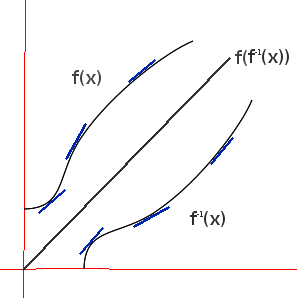
\includegraphics[scale=0.6]{figures/invfuncthm}
\end{figure}

We wish to generalize this statement to functions of multiple variables.
\begin{ldefn}
  We call $f|_u$ a restriction of $f$ at $u$; we only consider $f$ on the subset $u$ of the domain and its image from $u$.
  More precisely, using the definition of functions as certain subsets of cartesian products, we define $f|_u:=\{(x,y)\in f$ s.t. $x\in u\}$.
\end{ldefn}

\begin{thm}[Inverse function theorem for functions of several variables]
  Given
  \begin{enumerate}
  \item $f: u \to \RR^n. u \subset \RR^n$ ($u$ is an open n-ball)
  \item $f$ is differentiable on $u$, or, equivalently, $f|_u$ is differentiable
  \item $Df: u \to L(\RR^n)$ is continuous.
  \item $Df(x_0)$ is invertible $x_0 \in u$, or, equivalently, that the jacobean $J_f(x_0)$ is invertible in $M^{n\times n}$
  \end{enumerate}
  Then $\exists$ neighbohrhood $u_0 \subset u$ of $x_0$ so that $f|_{u_0}$ is bijective onto its image $v_0 = f(u_0)$ (invertible), the inverse $g = (f|_{u_0})^{-1}$ is also differentiable on $v_0$ and $\forall y = f(x) \in v_0$
  $$Dg(y) = (Df(x))^{-1}$$
  or, equivalently
  $$J_g(y) = (J_f(x))^{-1}$$
\end{thm}

Proof sketch:
\begin{enumerate}[I]
\item $\exists u_0$ neighbourhood of $x_0$ such that $f|_{u_0}$ is bijective with inverse $g: v_0 \rightarrow u_0$, where $v_0 = f(u_0)$ (using \emph{Banach fixed point theorem})
\item $v_0$ is open
\item $g$ is differentiable on $v_0$ and $D_g(y) = (Df(g(y)))^{-1}, \forall y \in v_0$
\end{enumerate}

\begin{defn}
  A function defined from metric space $(\Set{X}, d)$ to itself $\kappa: \Set{X} \rightarrow \Set{X}$ is called a contraction if
  $$d(\kappa(x), \kappa(y)) < cd(x,y).\ \forall x, y \in \Set{X}.\ c \in [0, 1)$$
\end{defn}

\begin{rem}
  Intuitive picture of a contraction $\kappa$ involves  a function where the preimage always changes faster than the image; graph would be `flatter' the smaller $c$ is.
\end{rem}

\begin{ldefn}
  A complete metric space is a metric space where all cauchy sequences converge. i.e. $$((x_p) \in \Set{X} \implies \forall \epsilon > 0 . \ \exists N_\epsilon \in \NN : d(x_p, x_q) < \epsilon .\  \forall p, q \geq N_\epsilon) \implies x_p \underrightarrow{^{p\rightarrow \infty}} x \in \Set{X} $$
\end{ldefn}

\begin{thm}[Banach fixed point theorem]
  Let $(\Set{X}, d)$ be a complete metric space. If $\kappa: \Set{X} \rightarrow \Set{X}$ is a contraction mapping, then $\kappa$ has a unique fixed point $x \in \Set{X}$, i.e. a point $x \in \Set{X}$ where $\kappa(x) = x$.
\end{thm}

\begin{rem}
  Intuitive picture of Banach fixed point theorem: because $\kappa$ is a contraction (the preimage $x$ is always changing faster than the image $\kappa(x)$), you know that somewhere as you're moving towards either its maximal point (e.g: $+\infty$) or minimal point (e.g: $-\infty$) the value of $x$ will catch up to $\kappa(x)$
\end{rem}

\begin{proof}
  \begin{enumerate}
  \item Take some $x_1 \in \Set{X}$
  \item Define sequence $(x_p)$ inductively such that $x_{p+1} = \kappa^p(x_1).\ p \in \NN$
  \item Define inequality
    \begin{equation}
      \label{l8e0}
      d(x_{p+1}, x_p) \leq c^{p-1}d(x_2, x_1).\ p \in \NN.\ c \in [0, 1)
    \end{equation}
    where $c$ is the contraction constant for $\kappa$. 
  \item Proving above inequality by induction.
    \par Base case (p = k = 1):
    $$d(x_{1+1}, x_1) \leq c^{1-1}d(x_2, x_1)$$
    $$d(x_2, x_1) \leq (c^0)d(x_2, x_1) \implies d(x_2, x_1) = d(x_2, x_1)$$
    \par Inductive step (p = k + 1)
    $$d(x_{k+2}, x_{k+1}) = d(\kappa(x_{k+1}), \kappa(x_{k}))$$
    Since $\kappa$ is a contraction
    $$ = d(\kappa(x_{k+1}), \kappa(x_k)) \leq cd(x_{k+1}, x_k)$$
    Activate induction
    $$ \leq cc^{k-1}d(x_2, x_1) = c^kd(x_2, x_1)$$
  \item We will show the sequence $(x_p)$ is cauchy. Let $m, n \in \NN.\ m > n$
  \item By triangle inequality
    $$d(x_m, x_n) \leq d(x_m, x_{m-1}) + d(x_{m-1}, x_{m-2}) + \dots + d(x_{n+1}, x_n)$$
    By inequality (\ref{l8e0})
    $$\phantom{d(x_m, x_n) } \leq c^{m-2}d(x_2, x_1)+c^{m-3}d(x_2, x_1)+\dots + c^{n-1}d(x_2, x_1)$$
    $$\phantom{d(x_m, x_n) } = c^{n-1}d(x_2, x_1)\sum_{k=0}^{m-n-2}c^k$$
    $$\phantom{d(x_m, x_n) } \leq c^{n-1}d(x_2, x_1)\sum_{k=0}^{\infty}c^k = c^{n-1}d(x_2, x_1)\frac{1}{1-c}$$
    So finally
    $$d(x_m, x_n) = c^{n-1}\frac{d(x_2, x_1)}{1-c}$$
  \item Let $\epsilon = c^{N-1}\frac{d(x_2, x_1)}{1-c} > 0 \iff N = \lceil \log_c(\frac{\epsilon(1-c)}{d(x_2, x_1)})\rceil + 1$
  \item $\epsilon$ is arbitrary, so the sequence $(x_p)$ is cauchy. And since the metric space it is defined on, $(\Set{X}, d)$, is complete, it converges to some $x^* \in \Set{X}$.
  \item $\kappa$ is a contraction $\implies$ Lipschitz (with constant $< 1$) $\iff$ Lipschitz continuous. Thus we can have
    $$\kappa(\lim_{p\rightarrow \infty}x_p) = \lim_{p\rightarrow \infty}x_{p+1}$$
    $$\kappa(x^*) = x^*$$
    So $x^*$ is a fixed point of $\kappa$
  \item Suppose there exists another $y \in \Set{X}$ such that $\kappa(y) = y$, then
    $$0 \leq d(x^*, y) = d(\kappa(x^*), \kappa(y)) \leq cd(x^*, y)$$
    Since $|c| < 1$, $d(x^*, y) = 0$
    $$0 \leq d(\kappa(x^*), \kappa(y)) \leq 0$$
    $$x^* = \kappa(x^*) = \kappa(y) = y$$
    So $x^*$ is the unique fixed point.
  \end{enumerate}
\end{proof}


\begin{proof}[The inverse function theorem proof]
  \par :
  \begin{enumerate}[I]
  \item `$\exists u_0$ neighbourhood of $x_0$ such that $f|_{u_0}$ is bijective with inverse $g: v_0 \rightarrow u_0$, where $v_0 = f(u_0)$`
    \begin{enumerate}
    \item $A = Df(x_0) \in L(\RR^n)$ is invertible (by assumption), $\implies ||A|| \neq 0 \iff ||A^{-1}|| \neq 0$. Define
      $$\lambda = \frac{1}{2||A^{-1}||} > 0$$
    \item The differential map $Df: u \rightarrow L(\RR^n)$ is continuous in $x_0$ (by assumption); there exists (for the previously defined $\lambda > 0$) an open neighbourhood $u_0 \subset u$ of $x_0$ so that
      \begin{equation}
        \label{l8e1}
        ||Df(x) - Df(x_0)|| < \lambda \: \forall x \in u_0
        \end{equation}
    \item $\forall y \in \RR^n$ define a map $\kappa = \kappa_y: u \rightarrow \RR^n$ by
      \begin{equation}
        \label{l8e2}
        \kappa(x) = x + A^{-1}(y - f(x))
      \end{equation}
      \begin{rem}
        Contrary to what the notation suggests, we do not have $f(x) = y$ always; this is the case exactly when $x$ is a fixed point of $\kappa$. Note also here that $\kappa$ is not a contraction yet either, but the plan to show that $\kappa$ is a contraction.
      \end{rem}
    \item Finding the derivative of $\kappa$ by the chain rule
      $$D\kappa(x) = I + A^{-1}\circ(-Df(x)) = I - A^{-1}\circ Df(x) = A^{-1} \circ(A-Df(x))$$
    \item By properties of the operator norm we get $\forall x \in u_0$
      $$||D\kappa(x)|| = ||A^{-1} \circ(A-Df(x))|| \leq ||A^{-1}||\:||A-Df(x)||$$
      recall that $A = Df(x_0)$, and by inequality (\ref{l8e1}) is
      $$\phantom{||D\kappa(x)||} < ||A^{-1}||\lambda = ||A^{-1}||\frac{1}{2||A^{-1}||}=\frac{1}{2} < 1$$
    \item By proposition, since the differential is bounded $\implies$ map is Lipschitz. We have that $||\kappa(u) - \kappa(v)|| \leq \frac{1}{2}||u-v||, \:\:\forall u,v \in u_0 \implies $ $\kappa$ is a contraction.
    \item By Banach fixed point theorem, $\forall y \in \RR^n$, there is at most one fixed point $x\in u_0$ of $\kappa = \kappa_y \implies f(x) = y$. In particular, $\forall y \in v_0 = f(u_0)$ there exists exactly one \footnote{Banach fixed point theorem says that this implies that there exists \emph{at most one} x, but I think it's exactly one since it works for all $y$.} $x \in u_0$ with $f(x) = y \implies f|_{u_0}$ is injective $\implies f|_{u_0}$ is bijective.
    \end{enumerate}
    
  \item `$v_0$ is open`
    \begin{enumerate}
    \item Let $y_1 \in v_0$ and let $x_1 = f^{-1}(y_1)$.
    \item Since $u_0$ is open, $\exists \rho > 0$ so that closed ball $\overline{B(x_1, \rho)} = \{u\in \RR^n:||x_1-u|| \leq \rho\} \subset u_0$
    \item We will show that $B(y_1, \lambda \rho) \subset v_0$ which would imply that $v_0$ is open; we need to prove that
      $$||y - y_1|| < \lambda \rho = \frac{\rho}{2||A^{-1}||} \implies y\in v_0 = f(u_0)$$
    \item Let $y \in B(y_1, \lambda \rho)$. For $\kappa = \kappa_y$, we can have
      $$||\kappa(x_1) - x_1|| = ||A^{-1}(y-f(x_1))||$$
      by property of the operator norm is
      $$\leq ||A^{-1}||\ ||y-f(x_1)|| < ||A^{-1}||\lambda \rho = ||A^{-1}||\frac{\rho}{2||A^{-1}||} = \rho / 2 $$
      thus, $\forall x \in \overline{B(x_1, \rho)} := \overline{B}$,
      $$||\kappa(x)-x_1|| = ||\kappa(x) + (-\kappa(x_1) + \kappa(x_1)) - x_1||$$
      by triangle inequality
      $$\leq ||\kappa(x) - \kappa(x_1)|| + ||\kappa(x_1) - x_1|| \leq \frac{\rho}{2} + \frac{\rho}{2} = \rho$$
    \item But this means that $\kappa(\overline{B}) \subset \overline{B} \implies \kappa$ is a contraction of a complete metric space $\overline{B}$ with the euclidean metric.
    \item By Banach fixed point theorem, $\exists ! x \in \overline{B} : \kappa(x) = x \iff f(x) = y \iff y \in v_0 \implies v_0$ is open.
    \end{enumerate}
  \item `$g$ is differentiable on $v_0$ and $D_g(y) = (Df(g(y)))^{-1}, \forall y \in v_0$`
    \begin{enumerate}
    \item Let $g = (f|_{u_0})^{-1}$
    \item Since $f|_{u_0}$ is bijective, we have a one to one correspondance
      $$v_0 \rightarrow
      \begin{cases}
        y \phantom{+ k}\:\:\:\leftrightarrow\:\:\: x = g(y) \in u_0 \\
        y + k \:\:\leftrightarrow\:\: x + h = g(y+k) \in u_0 \\
      \end{cases}
      $$
    \item With $\kappa=\kappa_y$ defined in (\ref{l8e2}), and knowing $f(x) = y, f(x+h) = y+k$, we now have
      $$\kappa(x+h) - \kappa(x) = x + h + A^{-1}(y-f(x+h))-x-A^{-1}(y-f(x))$$
      $$\phantom{\kappa(x+h) - \kappa(x)} =h+A^{-1}(f(x)-f(x+h))=h-A^{-1}k$$
    \item We can have
      $$||h|| = ||x + h - x||$$
      since $\kappa$ is a contraction with constant $\frac{1}{2}$, it is
      $$\geq 2||\kappa(x+h)-\kappa(x)|| = 2||h-A^{-1}k||$$
    \item On the other hand
      $$||h|| = ||h-A^{-1}k + A^{-1}k||$$
      by triangle inequality is
      $$\leq ||h-A^{-1}k|| + ||A^{-1}k||$$
      by the previous inequality is
      $$\leq \frac{||h||}{2}+||A^{-1}k||$$
    \item Thus, $||A^{-1}k|| \geq \frac{||h||}{2}$ and finally
      $$||h|| \leq 2||A^{-1}k|| \leq 2||A^{-1}||\ ||k|| = \frac{2||k||}{2\lambda}$$
      \begin{equation}
        \label{l8e3}
        \implies ||h|| \leq \frac{||k||}{\lambda}
      \end{equation}
    \item We need to show that $Df(x)$ is invertible. Recall from property 6 of the operator norm that if $||B - A|| < \frac{1}{||A^{-1}||} \implies B$ is invertible. We have by inequality (\ref{l8e1}) (recall $A = Df(x_0)$)
      $$||Df(x) - A|| < \lambda = \frac{1}{2||A^{-1}||} < \frac{1}{||A^{-1}||}$$
      $implies Df(x)$ is invertible.
    \item Now to identify the differential of $g$ in $y=f(x)$, let $B=(Df(x))^{-1}$ (note $h = Ih = (BDf(x))h$)
      $$g(y+k) - g(y) - Bk = x+h-x-Bk = h-B(y+k-y)$$
      $$\phantom{g(y+k) - g(y) - Bk}= BDf(x)h - B(f(x+h) - f(x)) = -B(f(x+h)-f(x)-Df(x)h)$$
    \item Then $g$ is differentiable if following limit equals $0$ as $k \rightarrow 0$
      $$0 \leq \frac{||g(y+k) - g(y) - Bk||}{|k|} = \frac{1}{||k||}||B(f(x+h)-f(x)-Df(x)h)|| $$
      $$\leq \frac{||B||}{||k||}||f(x+h)-f(x)-Df(x)h||$$
      by inequality (\ref{l8e3}) is
      $$\leq \frac{||B||}{\lambda}\frac{f(x+h)-f(x)-Df(x)h}{||h||}$$
    \item As $k\rightarrow 0, h\rightarrow 0$ by inequality (\ref{l8e3}), and as $f$ is differentiable $\frac{||B||}{||k||}||f(x+h)-f(x)-Df(x)h||\ \underrightarrow{^{h\rightarrow 0}}\ 0$. $\frac{||B||}{\lambda}$ is a constant (by definition, $\lambda > 0$).
      So, finally,
      $$\lim_{k\rightarrow 0}\frac{||g(y+k) - g(y) - Bk||}{|k|} = 0$$
      thus $g$ is differentiable on $v_0$, and the differential is $B = (Df(x))^{-1}$.
    \end{enumerate}
  \end{enumerate}
\end{proof}

\begin{exam} of a map that is locally invertable in every point but not globally injective is a map of polar coordinates in the plane $f:(0,\infty) \times \RR \rightarrow \RR^2$ defined by $f(r, \theta) = \lrrvector{r \cos\theta}{r \sin\theta}$
  Take $r > 0, \theta \in \RR$, then $J_f(r, \theta) = \lttmatrix{\cos\theta}{-r\sin\theta}{\sin\theta}{r\cos\theta}$.
  $\det{J_f} = r\cos^2\theta + r\sin^2\theta \implies f$ is locally invertible in $(r, \theta)$
  But $f(r,\theta) = f(r, \theta + 2\pi)$, so $f$ is not injective.
\end{exam}

\begin{rem}
  One can strengthen the statement of the theorem by assuming $f$ is continuosly differentiable on all of $u$, then one can show (using property 7 of operator norm) that $g$ is also continuously differentiable. \footnote{Refer to Rudin}
\end{rem}
